\chapter{Introduction}

\section{Project Description}
This project is concerned with the alignment of multiple mammographic images using an image-alignment technique called Congealing [1]. The aim will be to implement image-alignment software which allows the user to not only choose standard Entropy to align the images as in [1], but also 2 different light-weight Fuzzy Entropy metrics for alignment - Non-Probabilistic and Hybrid entropy. The User will be able to generate 3 mean images of the input set, 1 for each metric. By utilising different alignment metrics on the same images the result should be a range of average images, which further may be used to ascertain the most useful entropy algorithm for the alignment of mammographic images.

Each input set of images must belong to the same tissue density category, but from different women, to allow the resulting mean image to be an accurate depiction of the average breast structure within that category. Once a mean image is constructed of each category, this should aid radiographers in their qualitative categorisation of a new patient's scans.

Simple and accurate categorisation is important due to the increased risk factors associated with denser tissue breasts. Therefore if a radiographer can be confident in their categorisation of a patient's breast tissue, should the patient fall within the higher risk category they can receive more frequent, specialised scans to detect any abnormalities quicker should they arise.

\begin{figure}[H]
  \center
  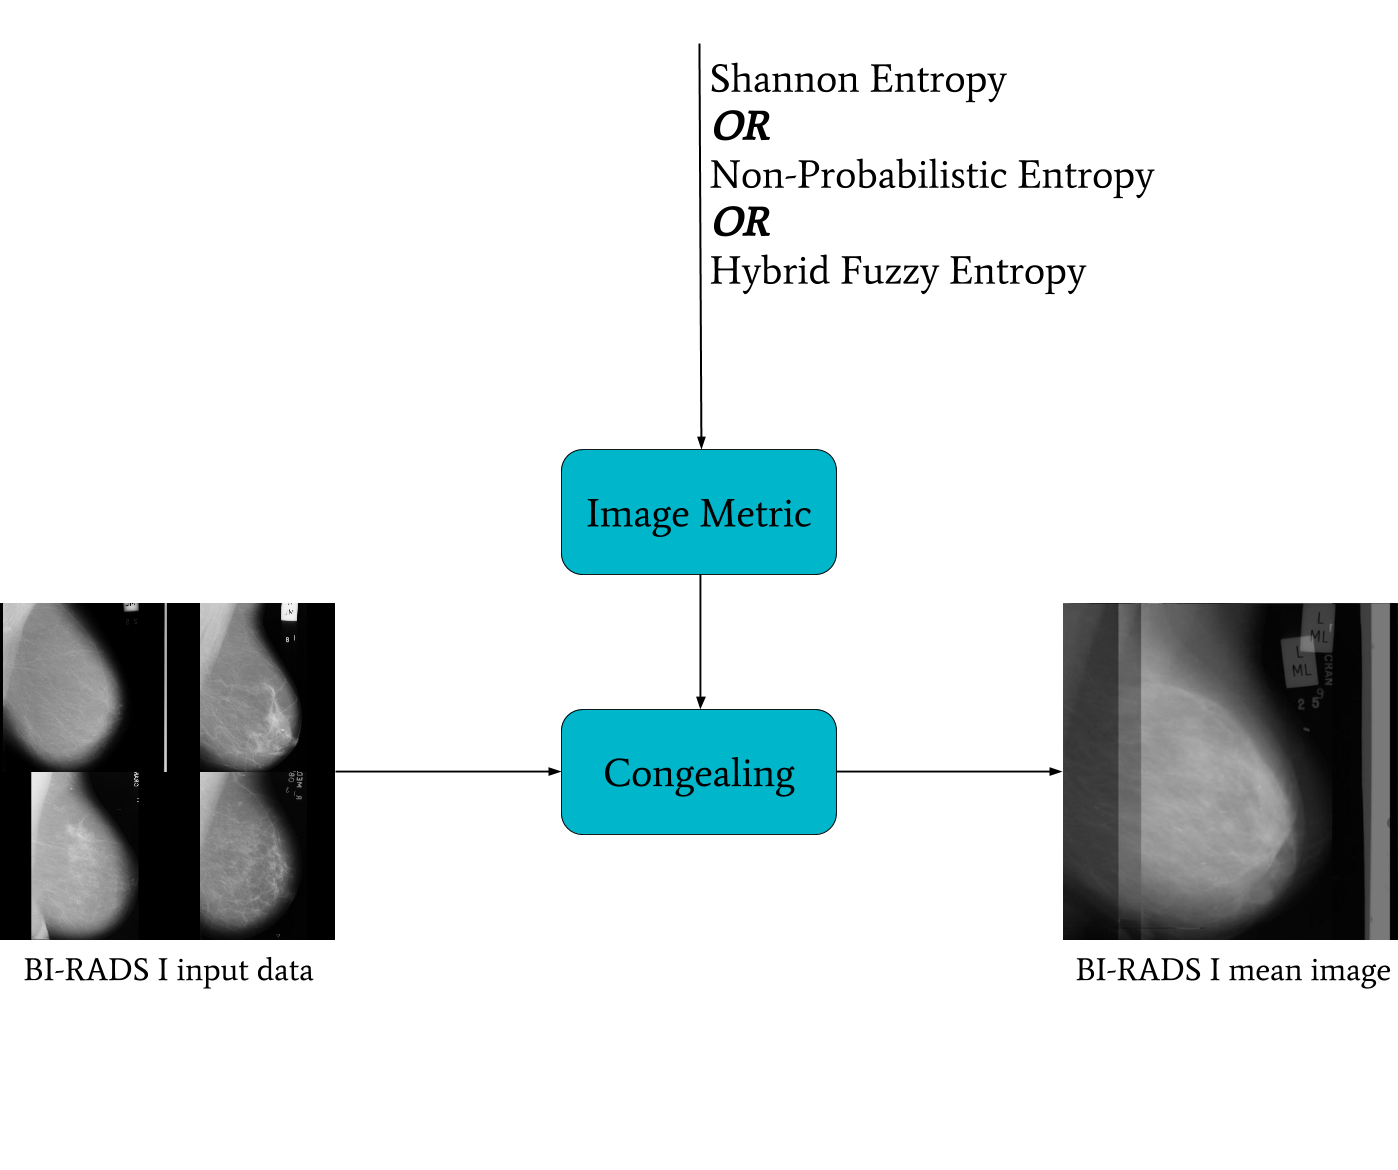
\includegraphics[scale=0.2]{/Users/lauracollins/Git/Major-Project/Documentation/Final/Introduction/project-desc-img/BI-RADS1.png}
  \caption{Graphical depiction of the project}
  \label{fig:project-desc-img}
\end{figure}
